
% This LaTeX was auto-generated from an M-file by MATLAB.
% To make changes, update the M-file and republish this document.

\documentclass{article}
\usepackage{graphicx}
\usepackage{color}
\usepackage{listings}
\usepackage[framed]{mcode}
\usepackage{fullpage}
\usepackage{hyperref}
\usepackage{amsmath}

\definecolor{lightgray}{gray}{0.5}
\setlength{\parindent}{0pt}

\begin{document}

    
    
%\section*{}

\begin{par}

\title{BE 521 - Homework 0\\{\normalsize Spring 2015}}
\author{Mike Lautman}
\date{\today}
\maketitle

\end{par}
\begin{par}

\section*{1. Unit Activity}

\end{par}
\begin{par}

\subsection*{1.1 IEEG portal spikes}
	\centering
	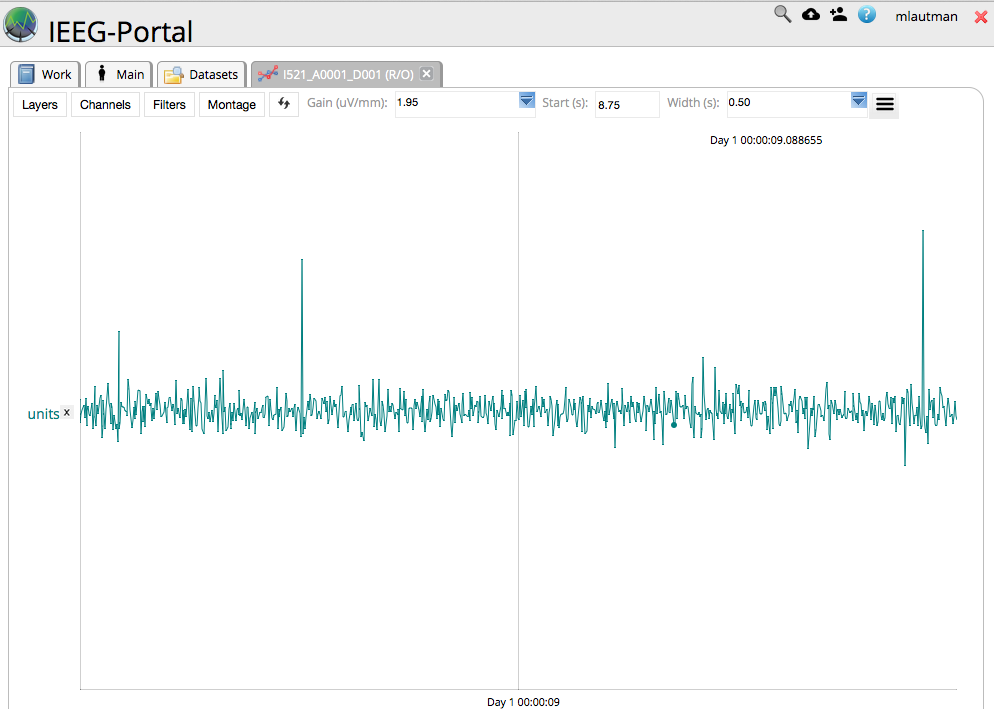
\includegraphics[width=4in]{three_peaks_IEEG.png}
	\\Figure 1. IEEG portal screenshot

\end{par}
\begin{par}

  \raggedright
  \subsection*{1.2 Grab data from IEEG}

\end{par}
\begin{lstlisting}
clear; clc; clf; close all;
dataset = 'I521_A0001_D001';
me = 'mlautman';
pass_file = 'mla_ieeglogin.bin';
[T,session] = evalc('IEEGSession(dataset, me, pass_file)');

session
\end{lstlisting}

\color{lightgray} \begin{lstlisting}
session = 

  <a href="matlab:help('IEEGSession')">IEEGSession</a>:

      server: 'ieeg.org'
    userName: 'mlautman'
        data: [1x1 IEEGDataset]

  <a href="matlab:methods(IEEGSession)">Methods</a>, <a href="matlab:IEEGObject.openPortalSite()">main.ieeg.org</a>

\end{lstlisting} \color{black}
\begin{par}

\subsection*{1.3 sample rate}

\end{par}
\begin{lstlisting}
data=session.data;
sample_rate = data.sampleRate
\end{lstlisting}

\color{lightgray} \begin{lstlisting}
sample_rate =

       32051

\end{lstlisting} \color{black}
\begin{par}

\subsection*{1.4 recording length}

\end{par}
\begin{lstlisting}
recording_length= data.channels(1).getNrSamples;
recording_length_s = recording_length/sample_rate
\end{lstlisting}

\color{lightgray} \begin{lstlisting}
recording_length_s =

    10

\end{lstlisting} \color{black}
\begin{par}

\subsection*{1.5a same window}

\end{par}
\begin{lstlisting}
s_s = 8.75;
e_s = s_s + .5;
s = max(round(s_s*sample_rate), 1);
e = min(round(e_s*sample_rate), recording_length);
vals = data.getvalues(s:e,1);
figure(1);

plot((s:e)./data.sampleRate, vals, 'color', 'b');

xlim([s_s, e_s]);
ylabel('Voltage (mV)', 'FontSize',10,'FontWeight','bold');
xlabel('Time (S)', 'FontSize',10,'FontWeight','bold');
title('Three spikes from IEEG dataset I521\_A0001\_D001', 'FontSize',12,'FontWeight','bold');
\end{lstlisting}


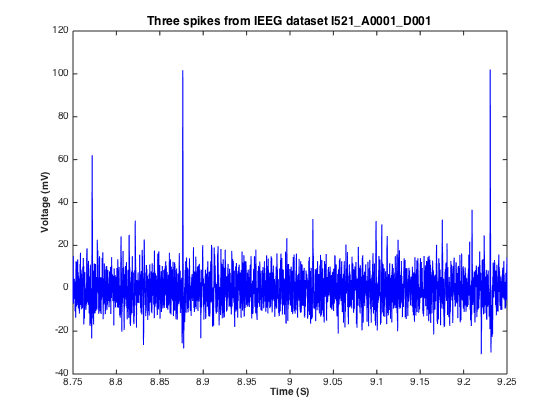
\includegraphics [width=4in]{BE521HW0_mlautman_01.png}
\begin{par}

\raggedright
\subsection*{1.5b Spikes}

\end{par}
\begin{lstlisting}
% NOTE: We define a spike as a locally convex region where the
% local maxima is greater than 5*std from the mean.

figure(2)
v_ave = mean(vals);
v_std = std(vals);
vals_spikes = (vals - v_ave > 5 * v_std) .* vals;
[pks,locs] = findpeaks(vals_spikes);
hold on


plot((s:e)./data.sampleRate, vals,'color', 'b' );
plot((s + locs)/sample_rate,pks, 'x', 'color','r');

xlim([s_s, e_s]);
ylabel('Voltage (mV)', 'FontSize',10,'FontWeight','bold');
xlabel('Time (S)', 'FontSize',10,'FontWeight','bold');
title('Three peaks from IEEG dataset I521\_A0001\_D001', 'FontSize',12,'FontWeight','bold');
\end{lstlisting}


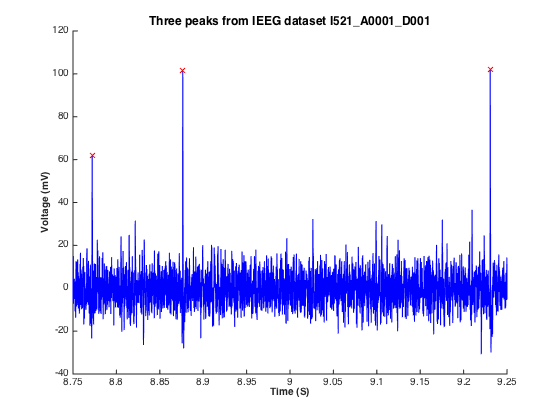
\includegraphics [width=4in]{BE521HW0_mlautman_02.png}
\begin{par}

\raggedright
\subsection*{1.5c Total Spikes in Recording}

\end{par}
\begin{lstlisting}
vals_all = data.getvalues(1:recording_length,1);
v_all_ave = mean(vals_all);
v_all_std = std(vals_all);
vals_all_spikes = (vals_all - v_all_ave > 5 * v_all_std) .* vals_all;
[pks_all,locs_all] = findpeaks(vals_all_spikes);
length(pks_all)

close all; clc;
\end{lstlisting}

\color{lightgray} \begin{lstlisting}
ans =

    42

\end{lstlisting} \color{black}



\end{document}
    
